%----------------------------------------------------------------------------------------
%	PACKAGES AND OTHER DOCUMENT CONFIGURATIONS
%----------------------------------------------------------------------------------------

\documentclass[11pt]{scrartcl} % Font size

\input{structure.tex} % Include the file specifying the document structure and custom commands
\usepackage{multirow}
\usepackage{array}
\usepackage{subcaption}
% Bar chart drawing library 
\usepackage{pgfplots} 
\usepackage{textcomp}
\usepackage{algorithm}
\usepackage{algpseudocode}


\usetikzlibrary{positioning}

% Define a macro to create a table with fixed column widths
\newcolumntype{C}[1]{>{\centering\arraybackslash}p{#1}}

\usepackage{hyperref}
\hypersetup{
    colorlinks=true,
    linkcolor=blue,
    filecolor=magenta,      
    urlcolor=cyan,
}

\definecolor{diffstart}{named}{Apricot}
\definecolor{diffincl}{named}{Green}
\definecolor{diffrem}{named}{Red}

\usepackage{listings}
  \lstdefinelanguage{diff}{
    basicstyle=\ttfamily\small,
    morecomment=[f][\color{diffstart}]{@@},
    morecomment=[f][\color{diffincl}]{+\ },
    morecomment=[f][\color{diffrem}]{-\ },
  }

\definecolor{codegreen}{rgb}{0,0.6,0}
\definecolor{codegray}{rgb}{0.5,0.5,0.5}
\definecolor{codepurple}{rgb}{0.58,0,0.82}
\definecolor{backcolour}{rgb}{0.95,0.95,0.92}
\definecolor{codeblue}{rgb}{0,0,0.8}

\lstdefinestyle{mystyle}{
    backgroundcolor=\color{backcolour},   
    commentstyle=\color{codegreen},
    keywordstyle=\color{codeblue},
    numberstyle=\tiny\color{codegray},
    stringstyle=\color{codepurple},
    basicstyle=\ttfamily\footnotesize,
    breakatwhitespace=false,         
    breaklines=true,                 
    captionpos=b,                    
    keepspaces=true,                 
    numbers=left,                    
    numbersep=5pt,                  
    showspaces=false,                
    showstringspaces=false,
    showtabs=false,                  
    tabsize=2
}

\lstset{style=mystyle}

%----------------------------------------------------------------------------------------
%	TITLE SECTION
%----------------------------------------------------------------------------------------

\title{	
	\normalfont\normalsize
	\textsc{Πανεπιστήμιο Πατρών, Τμήμα Μηχανικών ΗΥ και Πληροφορικής}\\ % Your university, school and/or department name(s)
	\vspace{25pt} % Whitespace
	\rule{\linewidth}{0.5pt}\\ % Thin top horizontal rule
	\vspace{20pt} % Whitespace
    {\Large Λογισμικό και Προγραμματισμός Συστημάτων Υψηλής Επίδοσης \\ \textbf{Final Project:} Function approximation with k-Nearest Neighbors}\\ % The assignment title
	\vspace{12pt} % Whitespace
	\rule{\linewidth}{2pt}\\ % Thick bottom horizontal rule
	\vspace{12pt} % Whitespace
}

\author{Ευάγγελος Λάμπρου \\UP1066519 \and Ιωάννης Παναρίτης \\UP1072632} % Your name

\date{} % Today's date (\today) or a custom date

%----------------------------------------------------------------------------------------
%	DOCUMENT
%----------------------------------------------------------------------------------------

\bibliographystyle{ieeetr}
\addto\captionsgreek{\renewcommand{\refname}{Αναφορές}}


\begin{document}

\maketitle 

% \tableofcontents

\section{Υλοποιήσεις}

\subsection{Σειριακή}

\subsubsection{Αρχική Υλοποίηση}

Στη σειριακή υλοποίηση το πρόγραμμα αποτελείται από τρία μέρη: 

\begin{enumerate}
    \item Φόρτωση των δεδομένων εκπαίδευσης (training) και ερωτήσεων (query).
    \item Εκτέλεση του αλγορίθμου KNN για κάθε ένα από τα σημεία ερώτησης.
    \item Παρουσίαση των αποτελεσμάτων (APE, MSE, $R^2$, χρόνοι εκτέλεσης)
\end{enumerate}

Για τον υπολογισμό του κάθε σημείου, ο KNN λειτουργεί ως εξής:

\begin{enumerate}
    \item Υπολογισμός της απόστασης του σημείου ερώτησης (query point) με όλα τα σημεία εκπαίδευσης.
    \item Επιλογή των $k$ σημείων με τη χαμηλότερη απόσταση από το query point. (γίνεται sorting πάνω στον πίνακα των αποστάσεων)
    \item Πρόβλεψη της τιμής του σημείου ερώτησης με βάση τις τιμές των $k$ επιλεγμένων σημείων. (μέσος όρος, weighted average, κλπ)
\end{enumerate}

Εκτελώντας την σειριακή υλοποίηση από τον perf profiler έχουμε τα ακόλουθα αποτελέσματα:

\lstinputlisting[caption={Αποτελέσματα του \src{perf report x.txt q.txt} (χωρίς τις κλήσεις στη βασική βιβλιοθήκη C)}, label={lst:perf}]{./assets/report-serial.txt}

Φαίνεται πως το μεγαλύτερο ποσοστό του χρόνου βρίσκεται στις συναρτήσεις \src{compute\_max\_pos} και \src{compute\_dist}, οι οποίες με τη σειρά τους εκτελούνται 
μέσα από την \src{compute\_knn\_brute\_force}. Συνεπώς, στόχος μας είναι η παραλληλοποίηση του \src{compute\_knn\_brute\_force}.

\subsubsection{Διαχείριση των δεδομένων}

Στην αρχική υλοποίηση του πργράμματος για κάθε query διαβαζόταν το επόμενο σημείο από το αρχείο \src{q.txt}. 
Ωστόσο, αυτό έχει ως αποτέλεσμα την δυσκολία παραλληλοποίησης του υπολογισμού των queries (δηλαδή το να υπολογίζονται πολλά queries ταυτόχρονα).
Έτσι, μετατρέπουμε το αρχείο \src{q.txt} σε έναν πίνακα στη μνήμη, ώστε να μπορούμε να προσπελάσουμε τα σημεία ερώτησης με την σειριακή σειρά που έχουν στο αρχείο.
Τελικά, έχουμε την επιλογή είτε να υλοποιήσουμε τα βήματα του αλγορίθμου KNN, ή να τρέχουμε πολλούς ξεχωριστούς αλγορίθμους KNN παράλληλα.

% create a figure with two subfigures
% the first subfigure should be the diagram you created above
% the second subfigure should be empty
% the two subfigures should be side by side
% the two subfigures should be centered in the page
\begin{figure}[H]
    \centering
    \begin{subfigure}[t]{0.4\textwidth}
        \centering
        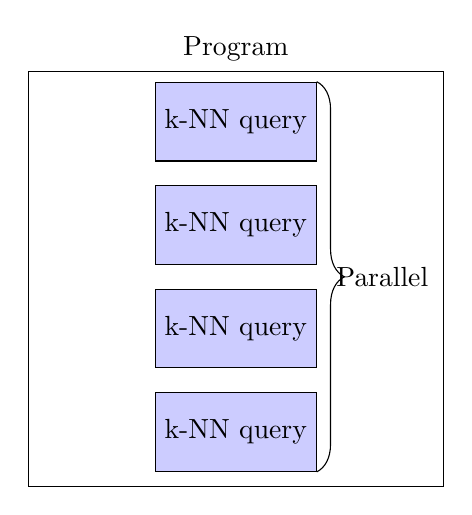
\begin{tikzpicture}
            \node [draw, minimum width=15em, minimum height=15em, label=above:Program] (program) at (0,0) {};
            \node [draw, fill=blue!20, minimum width=1cm, minimum height=1cm] (query1) at (0, 2)  {k-NN query};
            \node [draw, fill=blue!20, minimum width=1cm, minimum height=1cm, below=.3cm of query1] (query2)  {k-NN query};
            \node [draw, fill=blue!20, minimum width=1cm, minimum height=1cm, below=.3cm of query2] (query3)  {k-NN query};
            \node [draw, fill=blue!20, minimum width=1cm, minimum height=1cm, below=.3cm of query3] (query4)  {k-NN query};

            \draw [decorate, decoration = {brace, amplitude=10pt}] (query1.north east) -- (query4.south east)  node [midway, label=right:Parallel] {};
        \end{tikzpicture}
        \caption{Παραλληλοποίηση επιπέδου query.}
    \end{subfigure}
    \begin{subfigure}[t]{0.4\textwidth}
        \centering
        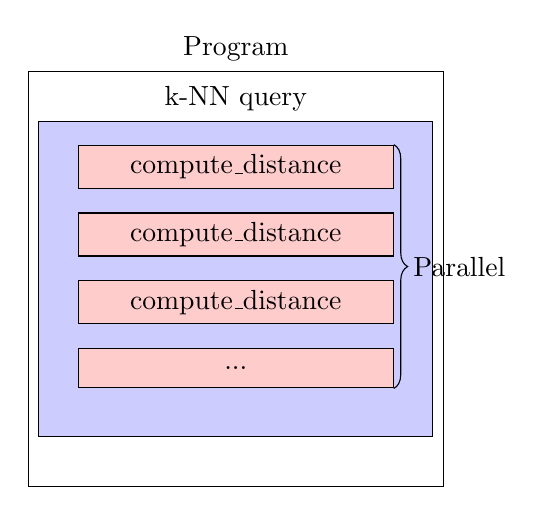
\begin{tikzpicture}
            \node [draw, minimum width=15em, minimum height=15em, label=above:Program] (program) at (0,0) {};
            \node [draw, fill=blue!20, minimum width=5cm, minimum height=4cm, label=above:k-NN query] (KNN) at (0, 0)  {};
            % draw 3 red rectangles inside the blue rectangle
            \node [draw, fill=red!20, minimum width=4cm, minimum height=.5cm, below=.3cm of KNN.north] (point1) {\src{compute\_distance}};
            \node [draw, fill=red!20, minimum width=4cm, minimum height=.5cm, below=.3cm of point1] (point2)  {\src{compute\_distance}};
            \node [draw, fill=red!20, minimum width=4cm, minimum height=.5cm, below=.3cm of point2] (point3)  {\src{compute\_distance}};
            \node [draw, fill=red!20, minimum width=4cm, minimum height=.5cm, below=.3cm of point3] (point4)  {...};

            \draw [decorate, decoration = {brace, amplitude=5pt}] (point1.north east) -- (point4.south east)  node [midway, label=right:Parallel] {};
        \end{tikzpicture}
        \caption{Παραλληλοποίηση του αλγορίθμου KNN}
    \end{subfigure}
    \caption{Παραλληλοποίηση του της εφαρμογής σε επίπεδο query και σε επίπεδο αλγορίθμου}
\end{figure}

\subsubsection{Αλγόριθμος Ταξινόμησης}

Για την επιλογή των $k$ κοντινότερων σημείων πρέπει στην ουσία να
ταξινομήσουμε τις αποστάσεις και να επιλέξουμε τα πρώτα $k$ σημεία.
Ωστόσο, έτσι όπως είναι υλοποιημένη η ρουτίνα που υπολογίζει τις αποστάσεις και
τοποθετεί τιμές αποστάσεων και indexes στους πίνακες \src{nn\_d} και \src{nn\_x} αντίστοιχα, 
στην ουσία έχουμε στα χέρια μας ήδη τα $k$ κοντινότερα σημεία, απλά δεν είναι με αύξουσα σειρά απόστασης.
Αυτό βέβαια δεν έχει σημασία για το τελικό αποτέλεσμα.
Συνεπώς, μπορούμε να αφαιρέσουμε ολοκλληρωτικά τη ρουτίνα ταξινόμησης.

\subsubsection{Αναδιάταξη Πράξεων}

Παρατηρώντας τα αποτελέσματα του profiler, βλέπουμε πως αφιερώνεται αρκετός χρόνος στη συνάρτηση \src{compute\_max\_pos}.
Έτσι, αναλύοντας τον κώδικα παρατηρήσαμε πως η συνάρτηση αυτή χρησιμοποιείται στη συνάρτηση \src{compute\_distance} σε μεγαλύτερο 
βαθμό απ'ότι χρειάζεται.

\lstinputlisting[language=diff]{./assets/compute_max.c.diff}

Είναι προφανές, ότι το index για το πού πρέπει να τοποθετηθεί το εκάστοτε σημείο στο array δεν χρειάζεται να υπολογίζεται σε 
κάθε επανάληψη, παρά μόνο τις φορές όπου υπάρχει υποψήφιο νέο σημείο με κοντινότερη απόσταση.
Αυτή η \say{διόρθωση} δίνει σοβαρή επιτάχυνση στη σειριακή υλοποίηση.

\subsection{OpenMP}

Στην OpenMP υλοποίηση του προγράμματος, αρχικά χρησιμοποιήσαμε μερικά OMP directives
για να επιταχύνουμε μερικές από τις ρουτίνες του αλγορίθμου ΚΝΝ.
Ωστόσο, παρατηρώντας ότι η πλειοψηφία των loops τρέχουν για λίγες επαναλήψεις, δεν πετύχαμε σημαντική επιτάχυνση στο χρόνο ανά query.
Παραλληλοποιώντας όμως σε επίπεδο query, είχαμε μια σημαντική επιτάχυνση στο συνολικό χρόνο εκτέλεσης του προγράμματος.



\subsection{OpenACC}

Για την υλοποίηση με OpenACC κάναμε προσέγγιση παρόμοια με αυτή της OpenMP, δηλαδή
παραλληλοποιήσαμε ρουτίνες του αλγορίθμου KNN. 
Βασική διαφορά τώρα όμως είναι πως προκειμένου να δούμε μείωση στο συνολικό χρόνο εκτέλεσης έπρεπε 
να ελαχιστοποιήσουμε τις μεταφορές δεδομένων μεταξύ επεξεργαστή και κάρτας γραφικών.

\subsection{CUDA}

Για την υλοποίηση με CUDA ουσιαστικά επιταχύνουμε την ρουτίνα υπολογισμού της απόστασης του σημείου
query με όλα τα άλλα σημεία.
Ορίζουμε ένα kernel \src{compute\_dist} το οποίο υπολογίζει την απόσταση του σημείου query με όλα τα άλλα σημεία 
και αποθηκεύει τα αποτελέσματα σε ένα array.

\subsection{MPI}

Για την υλοποίηση με MPI αποφασίσαμε να παραλληλοποιήσουμε τα ίδια τα queries και όχι το κάθε query ξεχωριστά, 
ουσιαστικά το κάθε process θα εκτελεί όλα τα queries που του αντιστοιχούν.
Αυτό έγινε για να ελαχιστοποιήσουμε τις μεταφορές δεδομένων μεταξύ των διεργασιών, αφού δεν θα υπάρχει ανταλλαγή δεδομένων παρά μόνο στην εκκίνηση και στη λήξη του αλγορίθμου.

\subsubsection{MPI Cluster και OpenMP}

Επόμενος στόχος ήταν η δημιουργία ενός MPI cluster, όπου θα είχαμε παραπάνω από ένα μηχάνημα μέσα σε περιβάλλον LAN να εκτελούν τα queries.

Οι διεργασίες που εκτελούνται στον κάθε cluster μπορούν να παραλληλοποιηθούν περεταίρω..
Έτσι, αφού είχαμε τη βασική υλοποίηση με MPI, προσθέσαμε στον κώδικα παραλληλοποίηση με OpenMP στον κώδικα του αλγορίθμου k-NN.

Τα βήματα για να δημιουργήσουμε ένα MPI cluster είναι τα εξής:

\begin{enumerate}
\item Εγκατάσταση του MPI σε όλα τα μηχανήματα.
\item Εγκατάσταση του OpenMPI σε όλα τα μηχανήματα.
\item Εγκατάσταση του OpenSSH σε όλα τα μηχανήματα, ενεργοποίηση του SSH server και δημιουργία κατάλληλων ssh κλειδιών.
\item Εγκατάσταση του NFS \cite{nfs} σε όλα τα μηχανήματα, ενεργοποίηση του NFS server και
        δημιουργία κοινόχρηστου φακέλου. Εκεί θα βρίσκεται το εκτελέσιμο και τα
        δεδομένα που θα χρησιμοποιούνται.
\item Εκτέλεση του κώδικα στον κύριο κόμβο με την εντολή:
\begin{lstlisting}
mpirun -np 6 --host laptop:1,desktop:4,ioanna:1 ./myknn-mpi x.txt q.txt
\end{lstlisting}
\end{enumerate}

\begin{figure}
    \begin{center}
        \includegraphics[width=0.7\textwidth]{assets/mpi_cluster.png}
    \end{center}
    \caption{Ο MPI Cluster μας να τρέχει τον αλγόριθμο K-NN σε ασύρματο LAN δίκτυο σε τρία μηχανήματα.}
    \label{fig:}
\end{figure}

Όπως ήταν αναμενόμενο, ο συνολικός χρόνος εκτέλσης του αλγορίθμου αυξήθηκε.
Ωστόσο, ο χρόνος ανά query, έφτασε ταχύτητα ισάξια της OpenMP υλοποίησης, πράγμα που δεν μας κάνει εντύπωση αφού σε επίπεδο query οι δύο υλοποιήσεις είναι πανομοιότυπες.
Αυτό οφείλεται στη μεγάλη απόκλιση μεταξύ του memory bandwidth και του network bandwidth.
Ένα τυπικό laptop έχει memory bandwidth της τάξης των 10 Gb/s ενώ ένας κόμβος σε ένα cluster έχει network bandwidth της τάξης των 1 Gb/s.
Αυτό σημαίνει ότι ο αλγόριθμος θα εκτελείται γρήγορα στον εκάστοτε κόμβο, αλλά η μεταφορά των δεδομένων από τον κύριο κόμβο στους υπόλοιπους και το αντίστροφο θα είναι πολύ πιο αργή.

% setup ssh
% setup nfs
% change /etc/exports
% exportfs -a
% restart nfs
% from client: sudo mount -t nfs -o master:/home/vagozino/mpi
% run RUN_CMD="mpirun -np 4 --host laptop:0,desktop:4 ./diffusion2d_mpi $D $L $N $T $DT" 

% mpi 1 machine: 4.307 time/query 20.35ms 
% mpi 3 machines: 26.753 time/query 12.54ms

% create a bar plot for the total time for 1 machine and 3 machines
% create a bar plot for the time/query for 1 machine and 3 machines
\begin{figure}[H]
    \begin{center}
\begin{tikzpicture}
    \begin{axis}[
        xlabel={Αριθμός Μηχανημάτων},
        ylabel={Time (s)},
        xtick=data,
        xticklabels={32, 1024, 2048},
        ybar,
        enlarge x limits=0.15,
        bar width=10pt,
        legend style={at={(0.5,-0.20)}, anchor=north, legend columns=-1},
        legend entries={1 Machine, 3 Machines},
        ymajorgrids=true,
        y grid style=dashed,
        nodes near coords,
        nodes near coords align={vertical},
        nodes near coords style={anchor=north},
        every node near coord/.append style={yshift=-2pt},
        every axis plot post/.append style={fill=blue!20},
        ]
        \addplot coordinates {(32, 4) (1024, 15) (2048, 28)};
        \addplot coordinates {(32, 9) (1024, 15) (2048, 24)};
    \end{axis}
\end{tikzpicture}
    \end{center}
    \caption{Χρόνοι εκτέλεσης της υλοποίησης με τον κώδικα MPI να τρέχει σε 1 Μηχάνημα (4 slots) και 3 Μηχανήματα (6 slots)}
    \label{fig:cluster_times}
\end{figure}

\section{Μετρήσεις}

\section{Έλεγχος Αποτελεσμάτων}

Για τον έλεγχο αποτελεσμάτων βασιστήκαμε στις μετρήσεις που εμφανίζονται με την εκτέλεση του προγράμματος.
Στον παρακάτω πίνακα παραθέτουμε τις μετρήσεις με την κάθε υλοποίηση.

\begin{table}[H]
    \centering
    \begin{tabular}{|l|c|c|c|c|c|}
    \hline
        Implementation & APE   & MSE   & $R^2$ & Total Time & Avg Time/Query \\ \hline
        Serial         & 0.000 & 0.000 & 1.000 & 0.000      & 0.000          \\
        OpenMP         & 0.000 & 0.000 & 1.000 & 0.000      & 0.000          \\
        OpenACC        & 0.000 & 0.000 & 1.000 & 0.000      & 0.000          \\
        MPI            & 0.000 & 0.000 & 1.000 & 0.000      & 0.000          \\
        CUDA           & 0.000 & 0.000 & 1.000 & 0.000      & 0.000          \\
    \hline
    \end{tabular}

    \caption{Έλεγχος ορθότητας των αποτελεσμάτων.}
\end{table}



\bibliography{bibliography}

\end{document}
